\documentclass{article}

\usepackage[utf8]{inputenc}
\usepackage[T1]{fontenc}
\usepackage[french]{babel}
\usepackage{hyperref}
\usepackage{enumitem}
\usepackage{geometry}
\usepackage{graphicx}
\usepackage{float}  
\usepackage{caption}


\title{Rapport de Projet d'OS 1}
\author{David de Meester, Imrane Benaissa, Maxime Lauzeral}
\date{\today}



\begin{document}
\maketitle


\section{Contenu}
\label{rapport}

\begin{enumerate}
    \item \hyperref[introduction-et-presentation]{Introduction et présentation}
    \item \hyperref[construction-du-programme]{Construction du programme}
    \begin{enumerate}[label*=\arabic*.]
        \item \hyperref[Dépendances]{Dépendances}
        \item \hyperref[Installation]{Installation}
    \end{enumerate}
    \item \hyperref[liste-des-fonctionnalites]{Liste des fonctionnalités}
    \item \hyperref[demonstration-en-pratique]{Démonstration en pratique}
    \begin{enumerate}[label*=\arabic*.]
        \item \hyperref[usage]{Usage}
        \item \hyperref[illustrations]{Illustrations}
        \begin{enumerate}
            \item \hyperref[fig:1]{Utilisateur bob exécute ./chat}
            \item \hyperref[fig:2]{Bob veut communiquer avec alice}
            \item \hyperref[fig:3]{Alice veut communiquer avec bob}
            \item \hyperref[fig:4]{Alice envoie un message à bob}
            \item \hyperref[fig:5]{Bob envoie un message à alice}
            \item \hyperref[fig:6]{Alice stoppe la conversation}
        \end{enumerate}
    \end{enumerate} 
    \item \hyperref[difficultes-rencontrees-solutions-apportees-choix-dimplementation]{Difficultés rencontrées, solutions apportées, choix d'implémentation}
    \begin{enumerate}[label*=\arabic*.]
        \item \hyperref[preambule-et-balbutiements]{Préambule et balbutiements}
        \item \hyperref[pipes-signaux-et-processus]{Pipes, signaux et processus}
        \item \hyperref[memoire-partagee-et-bot]{Mémoire partagée et bot}
    \end{enumerate}
    \item \hyperref[conclusion]{Conclusion}
\end{enumerate}


\newpage

\section{Introduction et présentation}
\label{introduction-et-presentation}

Ce projet de \textbf{INFO-F201} consiste en un petit programme permettant de discuter avec une personne ou un robot localement à l'aide de pipes nommés. 
Nous allons d'abord expliquer comment installer le programme, puis lister les fonctionnalités de ce dernier et montrer des exemples d'utilisation. 
Ensuite, nous discuterons des difficultés rencontrées et des solutions apportées en justifiant nos choix d'implémentation. 
Enfin, nous terminerons par une conclusion donnant notre sentiment global sur le projet.

\section{Construction du programme}
\label{construction-du-programme}


\subsection{Dépendances}
\label{Dépendances}
Le programme a été développé pour fonctionner sur une distribution Debian. 
Quelques préliminaires sont requis pour assurer une bonne installation. 
Ouvrez le terminal (\texttt{Ctrl+Alt+T}) et exécutez les commandes ci-dessous :

\begin{verbatim}
sudo apt update
sudo apt install build-essential
sudo apt install g++
sudo apt install make
\end{verbatim}

\subsection{Installation}
\label{Installation}
Nous avons décidé de créer un dépôt GitHub pour faciliter la mise en œuvre du projet. 
Comme les fichiers sources et un \texttt{Makefile} se trouvent dans le zip, vous pouvez compiler et exécuter le programme depuis le chemin de ce dernier à l'aide de \texttt{make}. 
Alternativement, si vous perdez le fichier zip, vous pouvez exécuter les commandes suivantes dans le répertoire de votre choix :

\begin{verbatim}
git clone https://github.com/kuzaiko/OS_PROJECT_1
cd OS_PROJECT_1
make
\end{verbatim}

\section{Liste des fonctionnalités}
\label{liste-des-fonctionnalites}

Le programme sans option permet de discuter avec un interlocuteur, de recevoir des messages et d'en envoyer.
Cependant, il est possible d'ajouter des options pour étendre les fonctionnalités du programme.
Les options supplémentaires proposées sont les suivantes :

\begin{verbatim}
#permet de recevoir les messages de l'interlocuteur uniquement sous certaines conditions
--manuel
\end{verbatim}


\begin{verbatim}
#permet de discuter avec un bot et d'exécuter les commandes ci dessous sensible à la casse
--bot
\end{verbatim}


\noindent \textbf{« liste »} : lister tous les fichiers du dossier de travail du robot ;\\
\textbf{« li FICHIER »} : lire le contenu du fichier « FICHIER » ou afficher une erreur en cas d’échec (p.ex., si le fichier est inexistant) ;\\
\textbf{« qui suis-je »} : donner le pseudonyme du destinataire ;\\
\textbf{« au revoir »} : terminer le robot avec le code de retour 0.\\

\section{Démonstration en pratique}
\label{demonstration-en-pratique}   


\subsection{Usage}
\label{usage}

Dans le répertoire où se trouve le fichier exécutable, exécutez :
\begin{verbatim}
./chat
\end{verbatim}


\subsection{Illustrations}
\label{illustrations}


\begin{figure}[H]
    \centering
    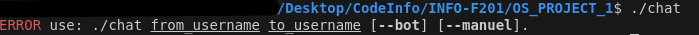
\includegraphics[width=\textwidth]{/home/pingwin/Desktop/CodeInfo/INFO-F201/OS_PROJECT_1/tex/1.png}
    \caption{Utilisateur bob exécute ./chat}
    \label{fig:1}
\end{figure}
\begin{figure}[H]
    \centering
    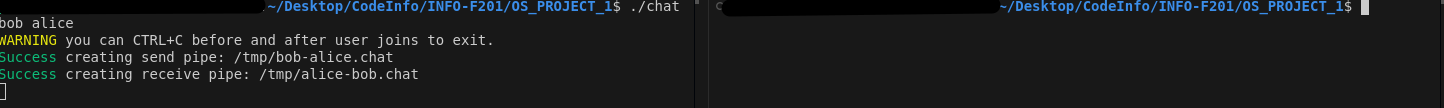
\includegraphics[width=\textwidth]{/home/pingwin/Desktop/CodeInfo/INFO-F201/OS_PROJECT_1/tex/2.png}
    \caption{Bob veut communiquer avec alice}
    \label{fig:2}
\end{figure}
\begin{figure}[H]
    \centering
    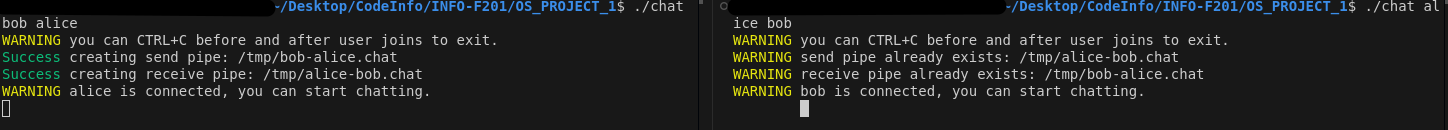
\includegraphics[width=\textwidth]{/home/pingwin/Desktop/CodeInfo/INFO-F201/OS_PROJECT_1/tex/3.png}
    \caption{Alice veut communiquer avec bob}
    \label{fig:3}
\end{figure}
\begin{figure}[H]
    \centering
    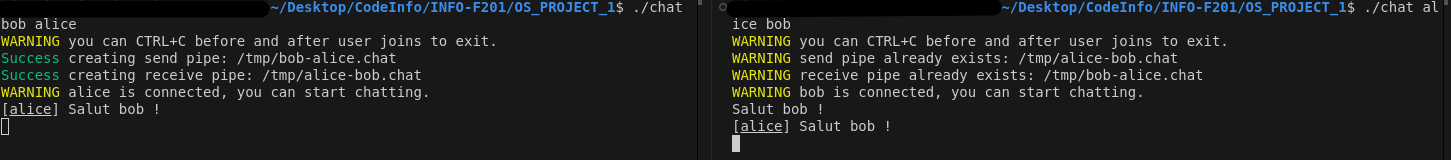
\includegraphics[width=\textwidth]{/home/pingwin/Desktop/CodeInfo/INFO-F201/OS_PROJECT_1/tex/4.png}
    \caption{Alice envoie un message à bob}
    \label{fig:4}
\end{figure}
\begin{figure}[H]
    \centering
    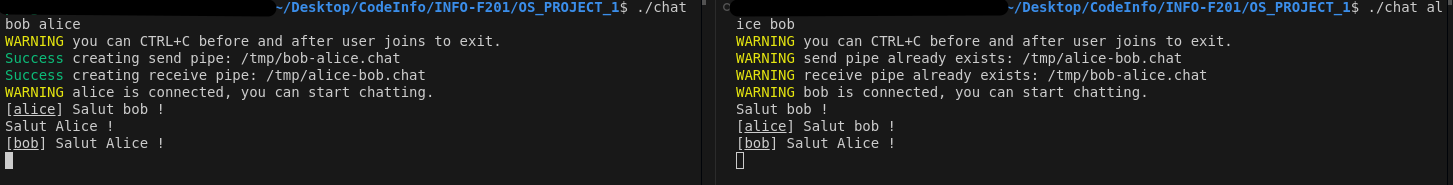
\includegraphics[width=\textwidth]{/home/pingwin/Desktop/CodeInfo/INFO-F201/OS_PROJECT_1/tex/5.png}
    \caption{Bob envoie un message à alice}
    \label{fig:5}
\end{figure}
\begin{figure}[H]
    \centering
    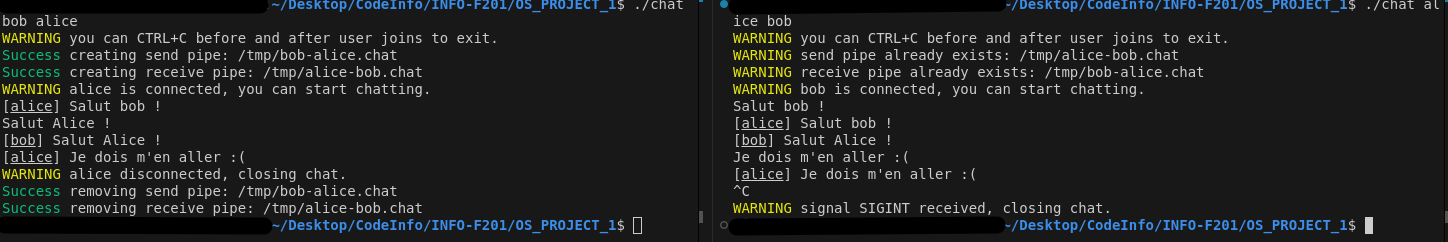
\includegraphics[width=\textwidth]{/home/pingwin/Desktop/CodeInfo/INFO-F201/OS_PROJECT_1/tex/6.png}
    \caption{Alice stoppe la conversation}
    \label{fig:6}
\end{figure}




\section{Difficultés rencontrées, solutions apportées, choix d'implémentation}
\label{difficultes-rencontrees-solutions-apportees-choix-dimplementation}

\subsection{Préambule et balbutiements}
\label{preambule-et-balbutiements}

L'utilisation de C n'était pas possible en raison de l'utilisation de certaines bibliothèques comme \texttt{<iostream>}, nous avons donc choisi d'utiliser C++.
La gestion des erreurs s'est faite via des macros dans un fichier \texttt{header} pour permettre une meilleure lisibilité.
Le soucis d'organisation nous a également préoccupés ; nous avons opté pour une structure modulaire séparant les fonctions, 
les classes et le \texttt{main} dans différents fichiers et créé un dossier supplémentaire contenant les différents \texttt{headers}.
Nous avons trouvé l'idée intéressante de créer certaines variables globales pour faciliter la communication entre les processus et d'également les mettre dans un \texttt{header}.

\subsection{Pipes, signaux et processus}
\label{pipes-signaux-et-processus}


Après avoir trouvé un début de structure, nous avons commencé à travailler sur les erreurs d'arguments et les pipes nommés. 
Nous avons trouvé élégant de créer une classe pour gérer la création, l'ouverture et la suppression des pipes.
Nous avons essayé au maximum de gérer les erreurs et de les afficher pour permettre à l'utilisateur de comprendre ce qui ne va pas.
De plus, nous avons utilisé des signaux pour gérer les interruptions de l'utilisateur et la déconnexion de l'interlocuteur.
Dans le premier cas, nous avons géré \texttt{SIGINT} dont le processus père s'occupe et dans le second cas, nous avons utilisé un \texttt{SIGPIPE} 
que le processus enfant appelle pour informer le père de la déconnexion de l'interlocuteur. 
Nous avons fait attention de fermer les pipes avant de les supprimer.

\newpage

\subsection{Mémoire partagée et bot}
\label{memoire-partagee-et-bot}


À la suite de la création de pipes, de la gestion des signaux et des processus, nous sommes passés au développement du mode manuel et du bot.
Nous avons utilisé \texttt{shm\_open} pour permettre le partage de mémoire entre les processus et avons choisi d'utiliser 4096 bytes pour la quantité de mémoire partagée.
Tout simplement car dans le mode manuel, nous avons une limite imposée de 4096 bytes avant l'envoi automatique des messages stockés dans la mémoire partagée.
Pour ce qui est des 3 scénarios du mode manuel, seul le processus enfant affiche le cas où la limite est atteinte.
Dans les deux autres cas, le père s'occupe de l'affichage. (\texttt{SIGINT} reçu et envoi de message par l'utilisateur)
Nous avons géré le cas d'une fermeture de stdin (\texttt{CTRL+D}) pour permettre à l'utilisateur de quitter le programme.
Encore une fois, nous avons fait attention à la gestion des erreurs et à la bonne fermeture des pipes et de la mémoire partagée.\\

À ce stade, il ne restait plus qu'à implémenter le bot. Nous avons créé un script \texttt{Bash} permettant de simuler un bot et de répondre aux commandes spécifiques.
Nous avons utilisé \texttt{coproc} comme conseillé dans le pdf, afin de pouvoir gérer les entrées et sorties du programme chat.
Enfin, nous avons veillé à utiliser flush sur la sortie standard pour éviter les problèmes de buffering.



\section{Conclusion}
\label{conclusion}

En conclusion, ce projet nous a permis de mettre en pratique les notions vues en cours, de nous familiariser avec les pipes nommés, les signaux, la gestion des processus, la mémoire partagée et le scripting bash.
Nous avons rencontré des difficultés importantes quant à l'organisation du code et du travail d'équipe. Nous sommes parti dans une direction et avons fait des choix d'implémentation qui nous l'espérons, sont pertinents.
Le projet était très intéressant et le pdf de consignes était très détaillé, nous avons fait en sorte de le suivre au mieux.


\end{document}
